\documentclass[conference]{IEEEtran}
\IEEEoverridecommandlockouts

\usepackage{cite}
\usepackage[utf8]{inputenc}
\usepackage{amsmath,amssymb,amsfonts}
\usepackage{algorithmic}
\usepackage{graphicx}
\usepackage{textcomp}
\usepackage{xcolor}
\usepackage{lettrine}
\usepackage{caption}
\usepackage{listings}
\usepackage{fancyhdr}
\usepackage{hyperref}
\usepackage[T1]{fontenc}
\usepackage{blindtext}
\usepackage[most]{tcolorbox}
\usepackage[backend=biber,
	isbn=true,                     % ISBN nicht anzeigen, gleiches geht mit nahezu allen anderen Feldern
	sortlocale=de_DE,               % Sortierung der Einträge für Deutsch
%sortlocale=en_US,              % Sortierung der Einträge für Englisch
	autocite=inline,                % regelt Aussehen für \autocite (inline=\parancite)
	hyperref=true,                  % Hyperlinks für Ziate
	style=numeric,                     % Zitate als Zahlen [1]
%style=alphabetic               % Zitate als Kürzel und Jahr [Ein05]
%style=authoryear                % Zitate Author und Jahr [Einstein (1905)]
%style=LNI
]{biblatex}

\addbibresource{Literatur.bib}

\def\BibTeX{{\rm B\kern-.05em{\sc i\kern-.025em b}\kern-.08em
    T\kern-.1667em\lower.7ex\hbox{E}\kern-.125emX}}
    
\renewcommand{\figurename}{Abbildung}

\definecolor{codegreen}{rgb}{0,0.6,0}
\definecolor{codegray}{rgb}{0.5,0.5,0.5}
\definecolor{codepurple}{rgb}{0.58,0,0.82}
\definecolor{backcolour}{rgb}{0.95,0.95,0.92}
\definecolor{block-gray}{gray}{0.95}

\newtcolorbox{zitat}[1][]{%
	colback=block-gray,
	grow to right by=-1mm,
	boxrule=0pt,
	boxsep=0pt,
	breakable,
	enhanced jigsaw,
	borderline west={2pt}{0pt}{gray},
	colbacktitle={block-gray},
	coltitle={black},
	fonttitle={\large\bfseries},
	attach title to upper={},
	#1,
}

\lstdefinestyle{mystyle}{
    backgroundcolor=\color{white},   
    commentstyle=\color{codegreen},
    keywordstyle=\color{magenta},
    numberstyle=\tiny\color{codegray},
    stringstyle=\color{codepurple},
    basicstyle=\ttfamily\footnotesize,
    breakatwhitespace=false,         
    breaklines=true,                 
    captionpos=b,                 
    keepspaces=true,                                   
    numbersep=5pt,                  
    showspaces=false,
    showstringspaces=false,
    showtabs=false,                  
    tabsize=1
}

\lstset{style=mystyle}

\pagestyle{fancy}
\fancyhf{}
\fancyhead[RE,CO]{Seminar Neue Technologien, C++ und Performance, Hochschule Offenburg, WS 2021/22}
\fancyfoot[LE,RO]{Seite \thepage}

\begin{document}
	\author{William Mendat, Angewandte Informatik, Hochschule Offenburg}
	\date{\today}
	\title{C++ und Performance}
	\maketitle

	\begin{abstract}
	Schon seit mehreren Jahrzehnten begleitet uns Software und stellt somit einen signifikanten Bestandteil unseres Lebens dar. In beinahe jeder Lebenssituation heutzutage findet sich Software wieder, sei es nun in den unzähligen Mikrocontrollern eines modernen Autos, welches ein hightech Computer auf rädern darstellt oder ein Videospiel, um von einem langen Arbeitstag abzuschalten. Die Anforderungen an Applikationen wachsen dabei stetig, weshalb neben logischer Korrektheit vermehrt auch Geschwindigkeit von übergeordneter Bedeutung ist. Vor allem im Embedded Bereich bekommt die Geschwindigkeit eines Programms noch mal eine viel größere Bedeutung, da hier auch meist in Lebens gefährdeten Bereichen hantiert wird. Werden die letzten Jahrzehnte betrachtet, zeigt sich, dass die vorherrschende  Programmiersprache im Embedded Bereich C ist. Jedoch zeigt sich auch, dass ein Trend zur Programmiersprache C++ entwickelt wurde. 
\newline
Dieses Paper befasst sich mit C++, einer Programmiersprache, die ursprünglich von Bjarne Stroustrup im Jahr 1979 als eine Erweiterung von C entwickelt wurde. Genauer soll darauf eingegangen werden, wie mit C++ sehr performant programmiert werden kann. Dabei soll gezeigt werden, wie mit einfach Ticks die Performance verbessert werden kann.
\end{abstract}
	
	\vspace{12pt}
	\begin{IEEEkeywords}
		C++, Performance
	\end{IEEEkeywords}

	\section{Einleitung}
\lettrine{B}{ei} dem Gedanken an die Programmiersprache C++ erschauern viele Programmierer, sei
es nun der blutige Anfänger, der noch nie etwas mit Programmierung zu tun hatte, oder der
langjährig erfahrene Embedded Programmierer, der lieber auf seine bewährte Programmiersprache C
zurückgreift. Dabei stellt sich die Frage, woher die Abneigung gegen diese Sprache kommt, wenn
Sie doch Perfekt scheint mit Ihrer nähe zur Hardware und den Vorteilen einer hohen
Programmiersprache. Gut, die Antwort darauf ist simpel, denn C++ ist ein Fluch und ein Segen
zugleich. C++ ist die momentan mächtigste Programmiersprache und in keiner anderen
Programmiersprache bekommt der Programmierer so viele Freiheiten, jedoch ist dies wie alles im
Leben nicht um sonst, denn mit vielen Freiheiten kommt auch viel Verantwortung.
\newline
\newline
Dieses Paper soll sich jedoch nicht mit dem sicheren Programmieren von C++ beschäftigen, sondern
eher damit, wie C++ ausgenutzt werden kann, um sehr performante Software zu schreiben. Tatsache
ist nämlich, dass genau so Performanter, wenn nicht sogar noch performanteren Code geschrieben
werden kann wie in C, jedoch um dies zu erreichen, sollte sich an die ursprünglichen Prinzipien
von C++ gehalten werden. Eines der ersten und zudem auch wichtigsten Prinzipien ist das
\emph{zero overhead abstraction} Prinzip beziehungsweise, nicht für das zu Bezahlen, was nicht
gebraucht wird \cite{HandsOn}[vgl.]. Unterstrichen wird dies noch mit dem Zitat  "Technically,
C++ rests on two pillars. A direct map to hardware (initially from C) and zero-overhead
abstraction in production code (initially from Simula where it wasn´t zero overhead). Depart from
those and the language is no longer C++"\cite{ISOC++}.
		
		

	%\section{Die Programmiersprache Dart}
	"Dart is a client-optimized language for fast apps on any platform" \cite{b1}. Die Programmiersprache wurde in erster Linie dazu Entwickelt, den Entwicklern es relativ einfach zu machen eine App für die Unterschiedlichsten Plattformen mit nur einer Programmiersprache zu entwickeln.

	\section{Take Four Problem}
Kontrovers soll dieses Paper mit der Thematik beginnen, wann es akzeptabel ist, nicht
grundsätzlich auf Performance zu achten. Dazu soll das \emph{Take Four Problem} genauer
betrachtet werden. Was ist das \emph{Take Four Problem}? Nun das \emph{Take Four Problem} zeigt
sechs Qualitätsmerkmale an Software, die im folgenden Schaubild dargestellt werden:

\begin{figure}[h]
    \centering
    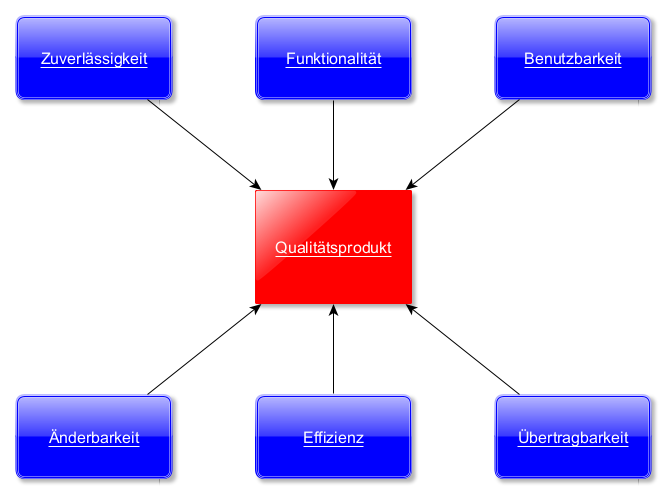
\includegraphics[width=0.5\textwidth]{bilder/ISO2}
    \caption[T4P]{Take Four Problem}
    \label{img:T4P}
\end{figure}

Das Problem, welches hier dargestellt werden soll, ist es, dass bei der Entwicklung von Software
sich auf vier der sechs Qualitätsmerkmale geeinigt werden muss, da sich manche Qualitätsmerkmale
gegenseitig ausschließen. Um ein konkretes Beispiel eines solchen Konfliktes zu nennen: Effizienz
und Zuverlässigkeit schließen sich gegenseitig aus, da Zuverlässigkeit viel auf Fehlertoleranz
baut und das Programm einfach performanter wird, wenn nicht jeder \emph{Pointer} auf \emph{null}
abgefragt wird. Auch die Wartbarkeit leidet meistens unter der Effizienz, was den Code dann zum
einen schlechter zu Lesen oder zu Erweitern ist.
\newline
\newline
Zu sehen ist also, dass es auf den Anwendungsfall stark ankommt. Ist das Produkt eine Webseite,
die ständig weiterentwickelt wird, dann ist es viel wichtiger, dass die Software leicht
erweiterbar geschrieben ist, zumal es bei einer Webseite nicht darauf ankommt, ob sie 20 oder 200
Millisekunden braucht, um zu laden.
\newline
\newline
Andersherum gesehen ist die Performance von Echtzeit kritischen Systemen von großer Relevanz. Bei
einem Airbag beispielsweise kann es lebensentscheidend sein, ob dieser innerhalb von 20 oder 200
Millisekunden rauskommt. Im Endeffekt muss im Vorfeld entschieden werden, welche Kriterien für
die Software als wirklich relevant erachtet werden.
	\section{Speicher Management}\label{sec:speicherman}
Der Speicher ist ganz klar die wichtigste Komponente beim Schreiben von einem Programm, denn ohne
den Speicher geht nichts. Da diese Komponente so enorm wichtig ist, muss auch besonders darauf
acht gegeben werden. Vor allem wenn es um die Performance eines Programms geht, kann beim
Speicher Management viel herausgeholt werden. In C++ ist dem Programmierer die Möglichkeit
gegeben, zwischen dem \emph{Stack} und dem \emph{Heap} zu entscheiden, wo dieser seine Objekte
speichert.

\subsection{Stack}
Dabei ist die Speicherung auf dem \emph{Stack} aus performanter Sicht sehr lukrativ, da dass
Speichern und Verwerfen von Objekten sehr schnell vonstattengehen kann. Jedoch ist nichts
umsonst und der \emph{Stack} kommt mit einigen Einschränkungen wie zum Beispiel der limitierten Größe,
die in Embedded Systems nicht besonders groß sein muss oder auch das keine dynamischen Objekte
dort gespeichert werden können \cite{C++HighPer2}[vgl.].

\subsection{Heap}
Sollen Objekte nun dynamisch gespeichert werden, dann kommt der Programmierer nicht drum herum,
diese Objekte auf dem \emph{Heap} abzulegen. Dies kann erreicht werden mithilfe der Verwendung von
der Funktion \emph{malloc} oder mit dem C++ Operator \emph{new}. Im Endeffekt wird \emph{malloc}
im \emph{new} Operator aufgerufen, der einzige Unterschied zwischen \emph{malloc} und \emph{new}
ist, dass bei \emph{new} noch der Konstruktor des Objektes aufgerufen wird. Das große Problem,
welches entsteht bei der Verwendung vom \emph{Heap}, ist, dass diese Operation sehr teuer aus
performanter Sicht ist. Zwei Faktoren, weshalb diese Operation so teuer ist, spielen dabei eine
Rolle. Zum einen ist das Anfordern von frischem Speicher an sich eine sehr teure Angelegenheit
und zum anderen ist die Platzierung der Daten komplett willkürlich, was zu sogenannten
\emph{Cache Misses} führen kann.
\newline
\newline
\emph{Cache Misses} sind unter anderem sehr kostspielig, wenn es um mehrdimensionale Arrays geht.
Im Folgenden wird als Beispiel ein dynamisches zweidimensionales Array auf dem \emph{Heap} abgelegt:

\begin{lstlisting}[
    caption={Anlegen eines Zweidimensionalem Array auf dem Heap},
    label=lst:Heap2DArray,
    frame=tlrb]
int main(int argc, char** argv){
	int** array2d = new int*[5];
	for (int i = 0; i < 5; ++i)
		array2d[i] = new int[5];
}
\end{lstlisting}

Nachdem das Array angelegt wurde, hat der Programmierer die Möglichkeit, sich die Adressen
anzusehen, wie im Folgenden durch eine Konsolenausgabe.

\begin{lstlisting}[
    caption={Mögliche Ausgabe der Adressen},
    label=lst:ArrayAdressen,
    language=bash]
arr2d[0]: 010B5188
arr2d[1]: 010B51C8
arr2d[2]: 010B52C8
arr2d[3]: 010B5308
arr2d[4]: 010BEE78
\end{lstlisting}

Zu sehen ist, dass die Adressen sehr weit auseinanderliegen, was dann sehr langsam sein kann,
wenn das Array beschrieben werden soll.

\subsection{Speicher auf dem Heap zuweisen}
Wie schon vorher erwähnt sind die \emph{Cache Misses} nicht die einzigen Performanzprobleme, die
entstehen, wenn Objekte auf dem \emph{Heap} gespeichert werden. Um Speicher vom \emph{Heap} zu
bekommen, muss der \emph{memory allocator} folgende Anforderungen erfüllen:

\begin{itemize}
    \item Es muss \emph{Multithreading} Unterstützen, da alle Threads nur auf den globalen
    \emph{Heap} zugreifen. Daher muss es auch eine Art von Synchronisation implementiert haben.
    \item Es muss effizient verschiedene Größen von Objekten zuweisen können.
    \item Es sollte sich nicht über die Zeit verschlechtern.
    \item Am Anfang eines Programmes wird vom Betriebssystem dem Programm speicher zur Verfügung
     gestellt und wenn dieser Aufgebraucht ist, dann muss es runter zum \emph{kernel}, um
     neuen Speicher anzufordern.
\end{itemize}

All diese Anforderungen und noch einige mehr müssen erfüllt werden! Zu sehen ist also, dass das
Speichern auf dem \emph{Heap} keines Falls trivial ist und mit bedacht einzusetzen ist
\cite{HandsOn}[vgl.].

\subsection{Benchmarking Stack vs. Heap}
Theorie ist gut, Praxis ist besser! Nach diesem Motto soll in dieser Sektion zwischen den beiden
Speicher Möglichkeiten verglichen werden, wie groß der Performance Unterschied tatsächlich ist.
Für diesen Zweck wurde ein zweidimensionales Array der Größe \emph{10x10} sowohl auf dem
\emph{Stack} als auch auf dem \emph{Heap} gespeichert und dessen Felder auf den Wert 2 gesetzt.
Dabei wurde die Compiler Optimierung ausgestellt, damit nichts Essenzielles vom Compiler bei
diesem Versuch wegoptimiert wird. Dieser Vorgang wurde dann \emph{N} Mal wiederholt und
resultierte in das folgende Ergebnis:

\begin{figure}[h]
    \centering
    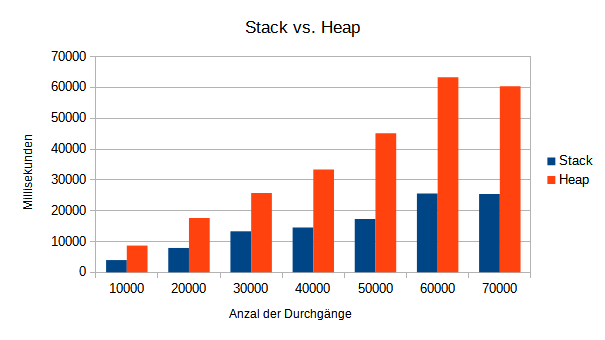
\includegraphics[width=0.5\textwidth]{bilder/StackvsHeap}
    \caption[StackvsHeap]{\emph{Stack} vs. \emph{Heap}}
    \label{img:StackvsHeap}
\end{figure}

Wie zu sehen ist, ist die \emph{Heapspeicherung} deutlich langsamer und der Performance
unterschied ist keinesfalls zu unterschätzen.
\newline
\newline
Ein interessanter Fakt, der zudem noch zu beobachten war, war, dass der Compiler auf der höchsten
Compiler Optimierungsstufe, in der Lage war, den Stack Code wegzuoptimieren. Dadurch wurde der
komplette Code für die Stack Implementierung verworfen und die gemessene Zeit resultierte in 0
Mikrosekunden.

\subsection{New Operator Überschreiben}
\begin{zitat}
    If we need dynamic memory and can't avoid allocations, we may have to write a custom memory
    manager that performs better for our specific needs \cite{C++HighPer2}.
\end{zitat}
In der vorhergehenden Sektion wurde für das Speichern auf dem \emph{Heap} die Standardimplementation von C
beziehungsweise C++ benutzt, dies ist jedoch nur eine generelle Funktion zum Zuweisen von
Speicher, deswegen auch auf nichts spezialisiert. C++ bietet dem Programmierer die Möglichkeit
seine eigene Implementation zu schreiben, indem der \emph{new} Operator überschrieben wird. Zum
Beispiel könnte am Anfang des Programms einmalig der gesamte Speicher, welches das Programm
ungefähr braucht, reserviert werden, um dann vom reservierten Speicher alle Objekte zu verwalten.
\newline
\newline
Neben der eigen Implementierung existieren natürlich noch externe alternativen zu der
Standardimplementierung von \emph{malloc}, wie zum Beispiel die Implementierung von Google, welche die
\emph{tcmalloc} Funktion zur Verfügung stellen.

\subsection{Zusammenfassung}
Abschließend kann gesagt werden, dass Speicher vom \emph{Heap} extrem kostspielig ist und hinter
dem \emph{new} Operator mehr steckt als manch einer vielleicht vermutet. Wie zudem auch zu sehen
war, ist die Möglichkeit gegeben, eine eigene Implementierung zu schreiben oder auf externe
Implementierungen zurückzugreifen. Alles im allem bleibt die Benutzung des \emph{Heap} sehr teuer
und es sollte, wann immer möglich mit dem \emph{Stack} gearbeitet werden.
	\section{Temporäre Objekte}\label{sec:tempobj}
Um temporäre Objekte verstehen zu können, sollte zuerst geklärt werden, was \emph{lvalues} und
\emph{rvalues} sind und worin diese zu Unterscheiden sind. Die Antwort darauf soll folgendes
Zitat liefern:
\begin{zitat}
    In concept (though not always in practice), rvalues correspond to temporary
    objects returned from functions, while lvalues correspond to objects you can refer to, either by
    name or by following a pointer or lvalue reference. A useful heuristic to determine whether an
    expression is an lvalue is to ask if you can take its address. If you can, it typically is. If
    you can’t, it’s usually an rvalue \cite{EffectiveC++}.
\end{zitat}
Wie zu sehen ist, resultieren \emph{rvalues} oft in temporären Objekten. Diese Objekte sind
insofern schlecht, da diese vom Compiler erzeugt werden, nur um Daten zu servieren, um dann sofort
wieder verworfen zu werden. Solch ein Verhalten frisst dann unnötigerweise Performance
\cite{HandsOn}[vgl].
\newline
\newline
Um ein solches Verhalten darzustellen, wird im Folgenden eine simple eigen Implementation der
\emph{String} klasse sowie die Klasse \emph{Person}, die eine \emph{const} Referenz übergeben im
Konstruktor übergeben bekommt, gezeigt:

\begin{lstlisting}[
    caption={Implementation einer String klasse},
    label=lst:String-klasse,
    language=C++,frame=tlrb]
class String {
public:
	String(const char* string) {
		printf("Created\n");
		m_Size = strlen(string);
		m_Data = new char[m_Size + 1];
		memcpy(m_Data, string, m_Size);
		m_Data[m_Size] = 0;
	}

	[...]

protected:
    uint32_t m_Size;
    char* m_Data;
};

class Person{
public:
	//Konstructor akzeptiert auch rvalues
	Person(const String& name) : m_Name(name) { }
private:
	String m_Name;
}
\end{lstlisting}

Wenn nun eine Instanz von Person mit einem \emph{rvalue} erstellt wird, dann wird zuerst ein
Objekt vom Typ \emph{String} erzeugt, nur um dann die Daten an \emph{m\_Name} zu kopieren. Im
späteren Verlauf dieses Papers wird noch auf das Kopieren von Objekten eingegangen. Jedoch kann
für den Moment gesagt werden, dass das Verhalten, ein Objekt lediglich zu erzeugen, nur um die
Daten dann weiterzureichen, sehr zulasten der Performance gehen.
	\section{Kopieren von Objekten}\label{sec:kopieren}
Sobald ein Objekt ein anderes Objekt zugewiesen wird, findet ein Kopiervorgang statt. Dabei
existieren zwei arten von Kopiermechanismen, einmal die \emph{flache} Kopie und die \emph{tiefe}
Kopie. Eine \emph{flache} Kopie ist eine Pseudo-Kopie, das bedeutet, dass hier nicht wirklich
Kopiert wird, sondern nur auf die Adresse des Objektes verwiesen wird, währenddessen ist eine
\emph{tiefe}, eine echte Kopie, bei der die Daten an eine neue Adresse geschrieben werden. Dies
ist insofern relevant, da bei dem Kopieren von einem Objekt der \emph{copy constructor}
aufgerufen wird, und dieser Standardmäßig eine \emph{flache} Kopie durchführt. Dieses Verhalten
soll im folgenden mit Hilfe der String klasse dargestellt werden.

\begin{lstlisting}[
    caption={Demonstration einer \emph{flachen} Kopie},
    label=lst:Flache-Kopie,
    language=C++,frame=tlrb]
int main(int argc, char** argv){
	String stringA = "Test";
	String stringB = stringA;
	stringB[1] = 'a';

	std::cout << "StringA: " << stringA << std::endl;
	std::cout << "StringB: " << stringB << std::endl;
}

//Output:
//StringA: Tast
//StringB: Tast
\end{lstlisting}

Wie klar zu erkennen ist, wurde durch die Veränderung von \emph{stringB} auch \emph{stringA}
verändert. Dieses verhalten ist jedoch sehr Problematisch, da nun zwei Objekte existieren, die
auf die gleiche Adresse verweisen und das Programm abstürzt beim versuch beide Objekte zu löschen
. Dies Passiert, weil versucht wird, Speicher freizugeben, der schon freigegeben wurde. Um dieses
unerwünschte verhalten zu umgehen, ist dem Programmierer die Möglichkeit gegeben, eine eigene
Definition für den \emph{copy constructor} zu schreiben. Für die eigen-implementierte String
klasse könnte der \emph{copy constructor} wie folgt aussehen:

\begin{lstlisting}[
    caption={String \emph{copy construtor}},
    label=lst:KopierKonstruktor,
    language=C++,frame=tlrb]
class String {
	[...]
    String(const String& other) {
        printf("Copied\n");
        m_Size = other.m_Size;
        m_Data = new char[m_Size + 1];
        memcpy(m_Data, other.m_Data, m_Size + 1);
    }
	[...]
};
\end{lstlisting}

Damit wurde erreicht, dass die beiden Objekte nun komplett voneinander unabhängig sind und das
Programm nicht abstürzt wenn beide Objekte gelöscht werden.
\newline
\newline
Jedoch ist gleichzeitig auch zu sehen, dass beim Kopieren neuer Speicher auf dem \emph{Heap}
angelegt werden muss, was wie im Kapitel \emph{\nameref{sec:speicherman}} sehr ineffizient ist. Das
bedeutet, dass jedes mal, wenn das String Objekt kopiert wird zum Beispiel beim Übergeben an eine
Funktion per \emph{Value}, dieser Vorgang unnötigerweise Performance in Anspruch nimmt. Im
späteren Verlauf dieser Arbeit wird noch ein C++ Feature gezeigt, welches eingesetzt werden kann
um unnötige Kopien zu vermeiden, jedoch für den Augenblick sollte gemerkt werden, dass ein Objekt
jedes mal per \emph{Referenz} an eine Funktion übergeben werden \cite{ChernoCopy}[vgl.].
	\section{Runtime Type Identification}\label{sec:rtti}
Runtime type Indentification kurz \emph{RTTI}, kann genutzt werden, um sicher zwischen
verschiedenen Typen in einer Klassenhierarchie zu \emph{casten}. Dabei verwendet \emph{RTTI}
Metadaten, die einer Klasse hinzugefügt werden, die dann zur Laufzeit verwendet werden können.
Mittels dem \emph{$dynamic\_cast$} Operator kann überprüft werden, ob zwischen einer Basisklasse
und einer abgeleiteten Klasse gecastet werden kann. Im Folgenden wird ein klassisches Beispiel
für die Verwendung von \emph{$dynamic\_cast$} demonstriert:
\begin{lstlisting}[
    caption={Demonstration von \emph{dynamic\_cast}},
    label=lst:Dynamic-Cast,
    language=C++,frame=tlrb]
class Stringbuilder : public String {
public:
	Stringbuilder(const char* string)
		:String(string) { }

    void PrintString() override {
    	std::cout << *this
       	<< " printed with Stringbuilder" << std::endl;
    }
};

int main(int argc, char** argv){
	String demo = new Stringbuilder("Demo");
	Stringbuilder* demoBuilder =
	dynamic_cast<StringBuilder*>(demo);

	if(!demoBuilder){
		//handle Error
	}
}
\end{lstlisting}

Hier kann nun geprüft werden, ob der \emph{cast} erfolgreich war, indem die Variable
\emph{demoBuilder} auf \emph{null} geprüft wird und wenn dem der Fall ist, dann war der
\emph{cast} nicht erfolgreich und es kann darauf reagiert werden.
\newline
\newline
Jedoch kommt es nun zu folgendem Problem: \emph{RTTI} fügt aus Performance Sicht unnötigen
\emph{overhead} hinzu und die Überprüfung bei \emph{$dynamic\_cast$} findet zur Laufzeit statt.
Wie schon in der Einleitung erwähnt, ist das \emph{zero overhead prinzip} eines der, wenn nicht
sogar das wichtigste Prinzip, welches hier klar verletzt wird. In dem Sinne sollte, sofern
möglich, \emph{RTTI} ausgeschaltet werden und auf Alternativen zurückgegriffen werden. Hier
existiert kein wissenschaftlicher Grundsatz, jedoch eine Möglichkeit, zumindest
\emph{$dynamic\_cast$} zu ersetzten, wäre die Verwendung einer \emph{Virtuellen Funktion}.
	\section{Fehlerbehandlungen}
Fehlerbehandlungen stehen der Performance eines Programms ständig im Weg, dies ist auch Logisch
zu erklären, da abgefangen und überprüft werden muss, ob es zu einem Fehler kam. Dafür muss
Programmcode hinzugefügt werden, der nicht essentiell für den eigentlichen Ablauf des Programms
ist. Dennoch kommt der Programmierer nicht drum herum Fehlerbehandlungen in seinem System zu
integrieren, da es immer zu unvorhergesehenen Fehlern kommen kann.

\subsection{Exceptions}
Um einen Fehler zu behandeln, kann der Programmierer einen Status Code zurückgeben und diesen
Überprüfen oder eine \emph{Exception} werfen und die Funktion die Potentiell eine
\emph{Exception} werfen könnte mit einem \emph{Try-Catch} Block umringen. Die Vorteile von
\emph{Exceptions} gegenüber von Status Codes, sind in dem folgenden Zitat schön zusammengefasst:

\begin{zitat}
    The use of exceptions isolates the error handling code from the normal flow of program
    execution, and unlike the error code approach, it cannot be ignored or forgotten. Also,
    automatic destruction of stack objects when an exception is thrown renders a program less likely to leak
    memory or other resources. With exceptions, once a problem is identified, it cannot be ignored –
    failure to catch and handle an exception results in program termination \cite{TechnicalReport}.
\end{zitat}

Wie zu sehen ist, bieten \emph{Excetions} nennenswerte Vorteile und haben somit auch eine
Daseinsberechtigung.
\newline
\newline
Obwohl klare Vorteile existieren, sind \emph{Exceptions} seit ihrer Einführung ein stark
umstrittenes Thema. Dies hat sich auch nach der Tabellen orientierten Optimierung, dass kein
Performance Verlust entsteht, wenn keine \emph{Exceptions} geworfen wird, nicht geändert. Der
Grund für die Umstrittenheit ist, dass \emph{Exceptions} gegen das \emph{zero-overhead prinzip}
verstoßen. Auch bei der Betrachtung der Performance eines Programms zeigen sich \emph{Exceptions}
als sehr Problematisch, da diese Dynamisch zur Laufzeit, zum Beispiel auf dem \emph{Heap}
erstellt werden müssen, was wie im Kapitel Speicher Management gezeigt, schon sehr teuer ist, und
anschließend noch der Dynamische Type der \emph{Exceptions} herausgefunden werden muss, was in
einem \emph{$dynamic\_cast$} resultiert. Ein weiteres Problem, welches mit der Verwendung von
\emph{Exceptions} kommt, ist dass nicht gesagt werden kann, wie lange es braucht bis eine
\emph{Exceptions} vollständig abgearbeitet ist. Dadurch kann die Situation entstehen, dass
während eine \emph{Exceptions} verarbeitet wird, eine andere geworfen wird und somit auch eine
unbestimmbare menge an Speicher gebraucht wird.\cite{HandsOn}

\subsection{Expected}
\emph{Exceptions} sind zwar sehr langsam, jedoch bringen sie wie vorher im Unterkapitel
\emph{Exceptions} erwähnt auch nennenswerte Vorteile gegenüber einfachen Status Codes. Deswegen
kann auf die Alternative von \emph{Expected} zurückgegriffen werden, welches einen Kompromiss
zwischen Status Codes und \emph{Exceptions} darstellt. \emph{Expected} wird durch
\emph{Templateklasse} repräsentiert, die Beispielhaft als Pseudocode, wie folgt aussehen könnte:
\newpage
\begin{lstlisting}[
    caption={Pseudocode einer Expected Klass\cite{OverheadExceptions}},
    label=lst:Expected-Klasse,
    language=C++,frame=tlrb]
template <class T>
class Expected {
private:
    union {
        T value;
        std::exception_ptr exception;
    };
public:
    Expected(const T& value) { ... }
    
    Expected(const std::exception_ptr& e) { ... }
    
    bool hasError() { ... }
    
    T getValue() { ... }
    
    std::exception_ptr getException() { ... }
};
\end{lstlisting}

Wie zu sehen ist, sind die zwei Variablen in einem \emph{union} gespeichert um das \emph{zero
overhead prinzip} nicht zu verletzen. Die Idee dahinter ist es, die \emph{Exception} nicht mehr
zu werfen, sondern diese wie einen erwarteten Wert zurück zu geben. Sollte die Funktion
erfolgreich durchlaufen, dann kann der erwartete Wert mittels der Funktion \emph{getValue()}
bekommen werden. Sobald jedoch ein Fehler aufkommt, wird dieser in der gleichen \emph{Instance}
gespeichert und mittels \emph{hasError()} kann dann überprüft werden, ob ein Fehler vorliegt.
Dadurch wurde erreicht, dass noch Metainformationen, zum Beispiel repräsentiert anhand von einem
\emph{String}, im Falle eines Fehlers zurückgegeben werden kann \cite{OverheadExceptions}[vgl.].
\newline

\begin{figure}[h]
    \centering
    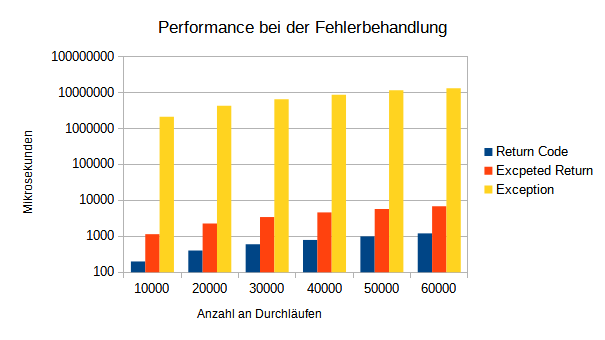
\includegraphics[width=0.5\textwidth]{bilder/Performance_Fehlerbehandlung}
    \caption[Fehlerbehandlung]{Performance bei der Fehlerbehandlung}
    \label{img:fehlerbehandlung}
\end{figure}

Abbildung \ref{img:fehlerbehandlung} zeigt den Performance unterschied zwischen der vorig
besprochenen \emph{Expected} Klasse als \emph{return} Wert und einen \emph{int} als \emph{return}
Wert, sowie der Fall, dass eine \emph{Exception} geworfen wird. Klar zu erkennen ist zwar dass
der Status Code immer noch wesentlich Performanter ist, jedoch ist der Unterschied zu
\emph{Exceptions} deutlich geringer.

\subsection{Zusammenfassung}
Trotz dessen, dass \emph{Exceptions} klare Vorteile bieten und durch Optimierungen, die
Performance nicht verschlechtern, wenn diese nicht geworfen werden, ist der Verlust an
Performance zu enorm, wenn diese geworfen werden. Große Firmen wie zum Beispiel Google haben
\emph{Exceptions} sogar komplett aus Ihren Projekten verboten. Durch die \emph{Templateklasse}
\emph{Expected} existiert eine lukrative Alternative, die wesentlich Performanter ist als
\emph{Exceptions}. Dennoch, wenn das Maximum an Performance in einem Programm herausgeholt werden
soll, dann sollte mit Status Codes gearbeitet werden.
	\section{Strings}\label{sec:strings}
Heutzutage ist es schon fast undenkbar und unmöglich, ein Programm ohne \emph{Strings} zu
schreiben. Sie sind ein fester Bestandteil bei so gut wie jeder höheren Programmiersprache
geworden. Viele Programmierer sehen diese deswegen auch als etwas sehr Leichtgewichtiges an. Dies
kommt
daher, dass Strings genauso behandelt werden wie primitive Datentypen, wie zum Beispiel \emph{int}
oder \emph{char}. Jedoch wäre es fatal anzunehmen, dass Operationen mit \emph{Strings} genauso
effizient geschehen, wie bei den primitiven Datentypen. Dies zeigt auch das folgende Zitat:

\begin{zitat}
    Strings are convenient because they automatically grow as needed to hold their contents. By
    contrast, C library functions (strcat(), strcpy(), etc.) act on fixed-size character arrays.
    To implement this flexibility, strings are allocated dynamically. Dynamic allocation is
    expensive compared to most other C++ features, so no matter what, strings are going to show
    up as optimization hot spots \cite{OptimizedC++}
\end{zitat}

\subsection{Probleme mit Strings}\label{subsec:stringprobleme}
\emph{Strings} ziehen viele Probleme mit sich, jedoch sind die zwei Größten Probleme, die
\emph{Strings} mit sich ziehen sind folgende:

\begin{itemize}
    \item \emph{Strings} werden auf dem \emph{Heap} gespeichert, was, wie im Kapitel
    \emph{\nameref{sec:speicherman}} gezeigt ein sehr Teurer Prozess ist.
    \item Dadurch, dass \emph{Strings} wie primitive Datentypen behandelt werden, verursachen
    \emph{Strings} viele Kopiervorgänge, was wie im Kapitel \emph{\nameref{sec:kopieren}} sehr
    suboptimal ist.
\end{itemize}

Um zu demonstrieren, wie problematisch diese zwei Punkte tatsächlich sind, soll die \emph{String}
klasse, die im Laufe dieses Papers vorgestellt wurde, um die \emph{+} und \emph{=} Operatoren
erweitert werden, wie im Folgenden gezeigt:
\newpage
\begin{lstlisting}[
    caption={String-Operatoren},
    label=lst:StringOperatoren,
    frame=tlrb]
	String& operator=(const String& other) noexcept {
		printf("Copied via =\n");
		if (this == &other)
			return *this;

		delete[] m_Data;
		m_Size = other.m_Size;
		m_Data = new char[m_Size + 1];
		memcpy(m_Data, other.m_Data, m_Size + 1);
		return *this;
	}

	String& operator+(const String& other) noexcept {
		this->operator+(other.m_Data);
	}

	String& operator+(const char* other) noexcept {
		printf("Copied via +\n");
		String temp = *this;

		delete[] m_Data;
		int other_Size = strlen(other);
		m_Size = temp.m_Size + other_Size;
		m_Data = new char[m_Size + 1];

		int i = 0;
		for (int j = 0; j < temp.m_Size; ++j, ++i)
			m_Data[i] = temp.m_Data[j];
		for (int j = 0; j < other_Size; ++j, ++i)
			m_Data[i] = other[j];

		m_Data[m_Size] = 0;
		return *this;
	}
\end{lstlisting}

Damit die beiden Operatoren so funktionieren, wie sie sollen, muss der Speicher für \emph{m\_Data}
mittels \emph{new} vergrößert werden. Darauf hin müssen die Daten entweder mit Standardfunktionen
wie \emph{memcpy} oder mit simplen \emph{for-schleifen}, kopiert werden.
\newline
\newline
Da nun die beiden Operatoren zur Verfügung stehen, kann nun mit der folgenden Sequenz die
Problematik zur Schau gestellt werden. Hierfür wird außerdem noch der \emph{new} Operator
überschrieben, um später zu überprüfen, wie oft die Funktion aufgerufen wurde.

\begin{lstlisting}[
    caption={String-Operationen},
    label=lst:StringOperationen,
    frame=tlrb]
static uint64_t Allocations = 0;

void* operator new(size_t size) {
	++Allocations;
	return malloc(size);
}

int main(int argc, char** argv)
{
	String demo = String("Hello") + " World" + "!";
	std::cout << "New called " << Allocations << " times" << std::endl;
	std::cin.get();
}
\end{lstlisting}
Wird die Sequenz betrachte, dann ist dies nichts Weltbewegendes, jedoch resultiert diese Sequenz
schließlich in diesen Output:

\begin{lstlisting}[
    caption={Ausgabe des String-Programms},
    label=lst:StringProgramm,
    language=bash]
Created
Copied via +
Copied
Copied via +
Copied
Copied
New called 6 times
\end{lstlisting}

Tatsächlich wurde für dieses doch sehr simple Programm sechsmal der \emph{new} Operator
aufgerufen. Ein Optimierungsansatz für dieses Problem sind \emph{\nameref{sec:move}}, die im
späteren Verlauf dieses Papers noch besprochen werden, jedoch ist dieses Verhalten aus Sicht der
Performance inakzeptabel und der Einsatz von \emph{Strings} sollte auf ein nötigstes beschränkt
werden.

\subsection{String Optimierungen}
Wie im Unterkapitel \emph{\nameref{subsec:stringprobleme}} zu sehen war, bringen \emph{Strings}
einige Probleme hinsichtlich der Performance mit sich. Jedoch ist die Tatsache, dass
\emph{Strings} Performance Probleme mit sich ziehen, kein Geheimnis und weit bekannt. Deswegen
wird stetig versucht, \emph{Strings} performanter zu machen. Im Folgenden werden aufgrund dessen
einige \emph{String} Optimierungen betrachtet, die im laufe der Jahre in den C++ Standard
hinzugefügt wurden.
\newline
\subsubsection{Small String Optimization}
Natürlich ist die \emph{std::string} klasse aus dem C++ Standard wesentlich Komplexer als die
eigen implementierte \emph{String} klasse aus diesem Paper und bietet auch mehr Features. So auch
wie das Feature names \emph{Small String Optimization}, welche mit \emph{C++11} in den C++
Standard kam. Wie in diesem Kapitel zu sehen war, müssen \emph{Strings} dynamisch auf dem
\emph{Heap} gespeichert werden. Durch \emph{Small String Optimization} werden \emph{Strings}, die
eine bestimmte Anzahl an Charakter nicht überschreiten, um genau zu sein, nicht größer als \emph{15}
Charakter, nicht auf dem \emph{Heap} sondern auf dem \emph{Stack} gespeichert. Dies ist durch die
folgende Demonstration zu erkennen:

\begin{lstlisting}[
	caption={Small String Optimization},
	label=lst:SmallString,
	frame=tlrb]
int main(int argc, char** argv)
{
	std::string string1 = "Hallo";
	std::cout << string1 << ": New called " << Allocations << " times" << std::endl;

	Allocations = 0;

	std::string string2 = "Hallo das ist eine Demo";
	std::cout << string2 << ": New called " << Allocations << " times" << std::endl;

	//Output
	//Hallo: New called 0 times
	//Hallo das ist eine Demo: New called 1 times
}
\end{lstlisting}
\newline
\subsubsection{std::string\_view}
Mit \emph{C++17} wurde \emph{std::string\_view} in den C++ Standard hinzugefügt und ermöglicht es
Programmierern, eine \emph{view} in einem \emph{String} zu bekommen. Eine \emph{view} sorgt
dafür, dass in einem schon vorhandenen \emph{String} reingeschaut werden kann. Wird nun das Beispiel
betrachte, das ein \emph{Substring} von einem \emph{String} benötigt wird, dann muss für diesen
\emph{Substring} ein eigener \emph{Buffer} auf dem \emph{Heap} erzeugt werden, um dann den Teil
zu kopieren. Mit Hilfe von \emph{std::string\_view} ist es nicht nötig, einen separaten
\emph{Buffer} zu erzeugen, sondern es wird lediglich auf die Adresse des \emph{Strings} gezeigt
und eine Anzahl an \emph{Bytes} übergeben, um den Teil des \emph{Substrings} zu definieren.
\newline
\subsubsection{Reserve}
Die \emph{Reserve} Funktion ist keine Eigenheit von \emph{std::string}, jedoch kann diese
Funktion genau so gut auch für \emph{Strings} benutzt werden. Mit \emph{Reserve} kann Speicher
auf dem \emph{Heap} reserviert werden, das bedeutet, dass wenn die Anzahl der \emph{Bytes} bekannt ist,
ist es nicht von Nöten jedes Mal nach einer Operation, mehr speicher anzufordern, sondern einmal
diese \emph{Bytes} zu reservieren und die Daten dann einfach reinzuschreiben. Angenommen, es
seien in einer \emph{Liste} beliebig viele \emph{Strings} vorhanden, und diese \emph{Strings}
sollen in  einem \emph{String} zusammen gefügt werden. Dann ist es tatsächlich performanter,
zuerst die gesamten \emph{Bytes} zu ermitteln, die Anzahl an \emph{Bytes} für den \emph{String} zu
reservieren und am ende erst die einzelnen \emph{Strings} zu vereinen. Im Folgenden wird ein
Diagramm gezeigt, welches den Unterschied mit und ohne \emph{Reserve} zeigt:
\begin{figure}[h]
	\centering
	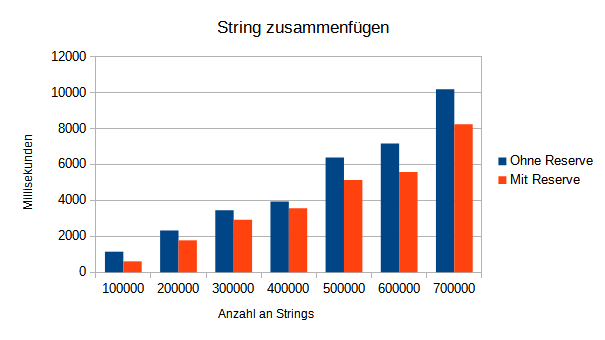
\includegraphics[width=0.5\textwidth]{bilder/StringReserve}
	\caption[StringsZusammenfügen]{Strings zusammenfügen}
	\label{img:StringsZusammenfügen}
\end{figure}
	\section{Fazit}\label{sec:fazit}
In diesem Paper wurde das Thema \emph{C++ und Performance} genauer behandelt. Dabei wurde im
ersten Abschnitt dieses Papers, auf das \emph{Take Four Problem} eingegangen, welches dann im
späteren verlauf, beim Kapitel \emph{\nameref{sec:fehlerbehandlung}} relevant wurde. Darüber
hinaus wurde auch dargestellt, was hinsichtlich der Performance, vermieden werden sollte. Zudem
wurden auch verschiedenste C++ Features vorgestellt, die allesamt die Performance eines
Programmes verbessern können. Zu allen Kapiteln wurden Codebespiele zur Demonstation
bereitgestellt und addierend noch die passende Erklärung wieso etwas funktioniert, wie es
funktioniert. Jedoch muss dazu auch gesagt werden, dass das Thema \emph{C++ und Performance} sehr
komplex und weitgreifend ist, deswegen soll dieses Paper nur dazu dienen einen kleinen Überblick
zu verschaffen. C++ ist eine sehr Komplexe sprache und wird noch komplexer beim Versuch
Performant zu schreiben aber durch die Einhaltung der Tipps, die in diesem Paper vorgestellt
wurden, ist schonmal gut angefangen.
	\section{Schlusswort}\label{sec:schlusswort}
Wie schon im \emph{\nameref{sec:fazit}} erwähnt, diente dieses Paper nur als einblick in dieses
doch recht komplexe Thema. Für diejenigen, die Interesse haben mehr über dieses Thema zu lernen
und sich weiter zu entwickeln, denen empfiehlt sich das Buch \emph{C++ High Performance 2nd
Edition} von Björn Andrist und Victor Sehr zu lesen. Das ist ein komplettes Buch mit vielen
Erklärungen für \emph{C++ und Performance} bis zum Stand von \emph{C++20}. Zudem ist die C++
Youtube reihe vom Youtuber \emph{TheCherno} für anfänger in C++ nur zu empfehlen, da dort von
Grund auf vieles erklärt wird.
	
	
	
	\printbibliography
	%\begin{thebibliography}{00}
    \bibitem{HandsOn} Krajewski, M. (2019): Hands-On High Performance Programming with Qt 5:
	Build cross-platform applications using concurrency, parallel programming, and memory
	management: Packt Publishing. Online verfügbar unter https://books.google
	.de/books?id=kiWGDwAAQBAJ.

    \bibitem{C++HighPer2} Andrist, B.; Sehr, V.; Garney, B. (2020): C++ High Performance: Master
	the Art of Optimizing the Functioning of Your C++ Code, 2nd Edition: Packt Publishing. Online
	verfügbar unter https://books.google.de/books?id=U9XczQEACAAJ.

    \bibitem{ISOC++} H. Hinnant, R. Orr, B. Stroustrup, D. Vandevoorde, M. Wong: Direction for
	ISO C++. Online verfügbar unter http://www.open-std
	.org/jtc1/sc22/wg21/docs/papers/2019/p0939r4.pdf, zuletzt geprüft am 25.08.2021.

    \bibitem{ISOIEC} Wikipedia: ISO IEC 9126. Online verfügbar unter $https://de.wikipedia
	.org/w/index.php?title=ISO/IEC_9126\&oldid=177832067$, zuletzt aktualisiert am 28.05.2018,
	zuletzt geprüft am 25.08.2021.

    \bibitem{EffectiveC++} Meyers, Scott (2015): Effective modern C++. 42 specific ways to
	improve your use of C++11 and C++14. Online-Ausg. Sebastopol, CA: O'Reilly Media. Online
	verfügbar unter http://proquest.tech.safaribooksonline.de/9781491908419.

    \bibitem{ChernoCopy} TheCherno (2017): Copying and Copy Constructors. Online verfügbar unter
	$https://www.youtube.com/watch?v=BvR1Pgzzr38\&list=PLlrATfBNZ98dudnM48yfGUldqGD0S4FFb\&index
	=45$,  zuletzt aktualisiert am 13.09.2017, zuletzt geprüft am 02.09.2021.

    \bibitem{TechnicalReport} Dave Abrahams (2006): Technical Report on C++ Performance. Online
	verfügbar unter http://www.open-std.org/jtc1/sc22/wg21/docs/TR18015.pdf, zuletzt geprüft am 06
	.09.2021.

    \bibitem{OverheadExceptions} Nayar, Amit (2020): Investigating the Performance Overhead of
	C++ Exceptions | PSPDFKit. Online verfügbar unter https://pspdfkit
	.com/blog/2020/performance-overhead-of-exceptions-in-cpp/, zuletzt geprüft am 06.09.2021.

\end{thebibliography}

\end{document}
